% Chapter 9

\chapter{Results on Radiative Corrections} % Chapter title

\label{ch:RC} % For referencing the chapter elsewhere, use \autoref{ch:name}

%----------------------------------------------------------------------------------------

The DJANGOH generator can have two usage : be used as a event generator inside a MC simulation or be used in a standalone way to compute radiative corrections. As we saw previously, DJANGOH as an event generator in TGEANT is giving consistent results. In addition, DJANGOH is able to compute radiative correction factors in bins of ($x$,$y$,$z$). For these reasons we were interested to calculate radiative correction factors with DJANGOH.

\section{Inclusive and Semi-Inclusive Radiative Correction factors}\label{sec:RCF}

The calculation of the inclusive radiative correction factors can be done by computing $\sigma_{Born}$ and $\sigma_{Born+o(\alpha)}$. A correct way to obtain these factors is the following :
%
\begin{equation}
  \eta(x,y)=\frac{\sigma_{Born}(x,y)}{\sigma_{Born+o(\alpha)}(x,y)}
  =\frac{\frac{\sigma_{Born,tot}*N_{Born}(x,y)}{N_{Born,tot}}}{\frac{\sigma_{Born+o(\alpha),tot}*N_{Born+o(\alpha)}(x,y)}{N_{Born+o(\alpha),tot}}}
\end{equation}
%
The results that are presented below are obtained with the TERAD $F_{2}$ and R parametrizations, which
describes accurately the behaviour of $F_{2}$ at low $Q^{2}$ \cite{BPnote} :

\begin{itemize}
\item $F^{p}_{2}(x,Q2)$ for $Q^2 > 0.2$ GeV$^2$ and $0.000035 < x < 0.85$, as obtained from a fit to the
world proton (and deuteron) data made by the SMC \cite{SMC}.
\item For $Q^2 < 0.2$ GeV$^2$, a phenomenological model of Badelek and Kwiecinski \cite{BK}, valid at $10^{-5} < x < 0.1$
and $0 < Q^2 < 1000$ GeV$^2$.
\item $R(x, Q^2)$ as parameterised by SLAC (newer version, called R1998 \cite{R1998}), valid for $Q^2 > 0.5$ GeV$^2$, extended
to lower values of $Q^2$, including the $R \simeq Q^2$ behaviour at $Q^2 = 0$.
\end{itemize}

All first order QED corrections are included except for quark line radiation. The reason why these corrections are not included is that these corrections are negligible except at large $x \geq 0.5$ and $Q^{2} \geq 10^3$ (GeV/$c$)$^2$, where the corrections reach the magnitude of barely one percent (see Fig.~\ref{fig:quarkline}). These corrections are often not subtracted inside the parametrization, thus they are already taken into account in the parametrization \cite{HubertF2Rad}. Nevertheless this is not the case for TERAD $F_2$.

\begin{figure}[htb]
\centerline{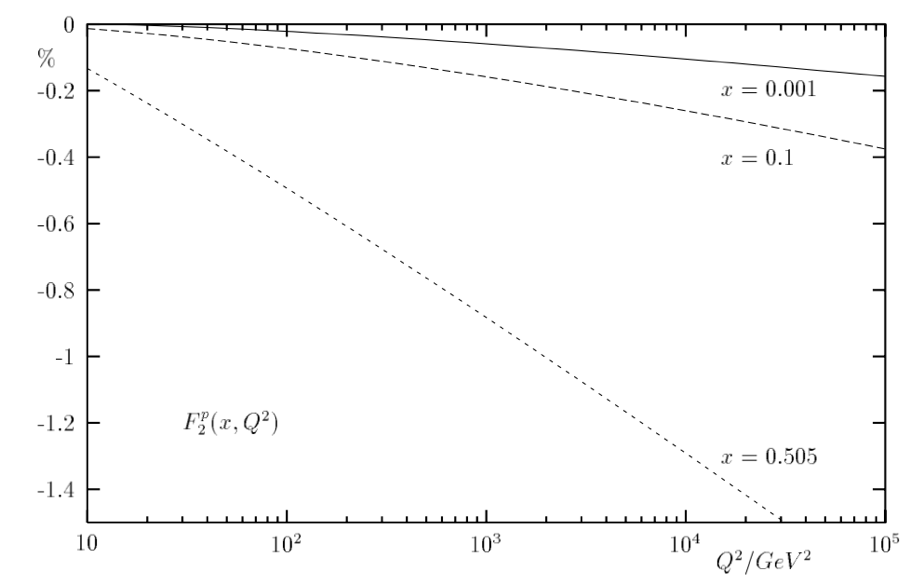
\epsfig{file=gfx/quarkline.png,width=12cm}}
\caption{$Q^2$ dependence of the quarkonic QED corrections (in percent) to the structure function $F^p_2$ for deep inelastic
lepton-proton scattering at $x=0.001$, $x=0.1$ and $x=0.505$. Figure taken from \cite{HubertF2Rad}.}\label{fig:quarkline}
\end{figure}

\subsection{Radiative correction factors : Effect on Multiplicities}\label{sec:RCFMult}

The calculation of the radiative correction factors to the multiplcities can be done by computing
$M^{h^{\pm}}_{Born}$, multiplicities obtained without radiative corrections, and $M^{h^{\pm}}_{Born+o(\alpha)}$,
multiplicities obtained with radiative corrections. The factors can be defined as :
%
\begin{equation}
  \begin{split}
    \eta^{h^{\pm}}(x,y,z)=\frac{M^{h^{\pm}}_{Born}(x,y,z)}{M^{h^{\pm}}_{Born+o(\alpha)}(x,y,z)} \\
     = \frac{N^{h^{\pm}}_{Born}(x,y,z)/N^{DIS}_{Born}(x,y)}{N^{h^{\pm}}_{Born+o(\alpha)}(x,y,z)/N^{DIS}_{Born+o(\alpha)}(x,y)}
  \end{split}
\end{equation}
%
where $N^h$ is the number of hadrons and $N^{DIS}$ the number of DIS events.


In the following plot, the cuts from the SIDIS analysis for the selection of DIS events and hadrons are used (see Chapter~\ref{ch:raw} for further details). The kinematical cuts used are :

\begin{itemize}
\item $0.004 \leq x \leq 0.4, x \in \{.004,.01,.02,.03,.04,.06,.1,.14,.18,.4\}$
\item $0.1 \leq y \leq 0.7, y \in \{.1,.15,.2,.3,.5,.\}$
\item $12 \leq p_h \leq 40$ GeV
\end{itemize}

Fig.~\ref{fig:hadz_ratio} exhibits the semi-inclusive radiative correction factor $\eta^{h^{\pm}}(x,y,z)$. This factor goes from $0$\% correction at low $z$ and low $y$ to $20$\% correction at high $z$ and high $y$. This dependence on $y$ and $z$ is expected (e.g. if a hadron has a high $z$ in a non-radiative event, consider the same event but with the radiation of a real photon, $\nu_{lep}$ will remain the same but the hadron will have in reality less energy available from the virtual photon, thus having $z_{had} \leq z_{lep}$, leading to less events in the high $z$ region for the multiplicities obtained with radiative correction).

\begin{figure}[!htb]
\centerline{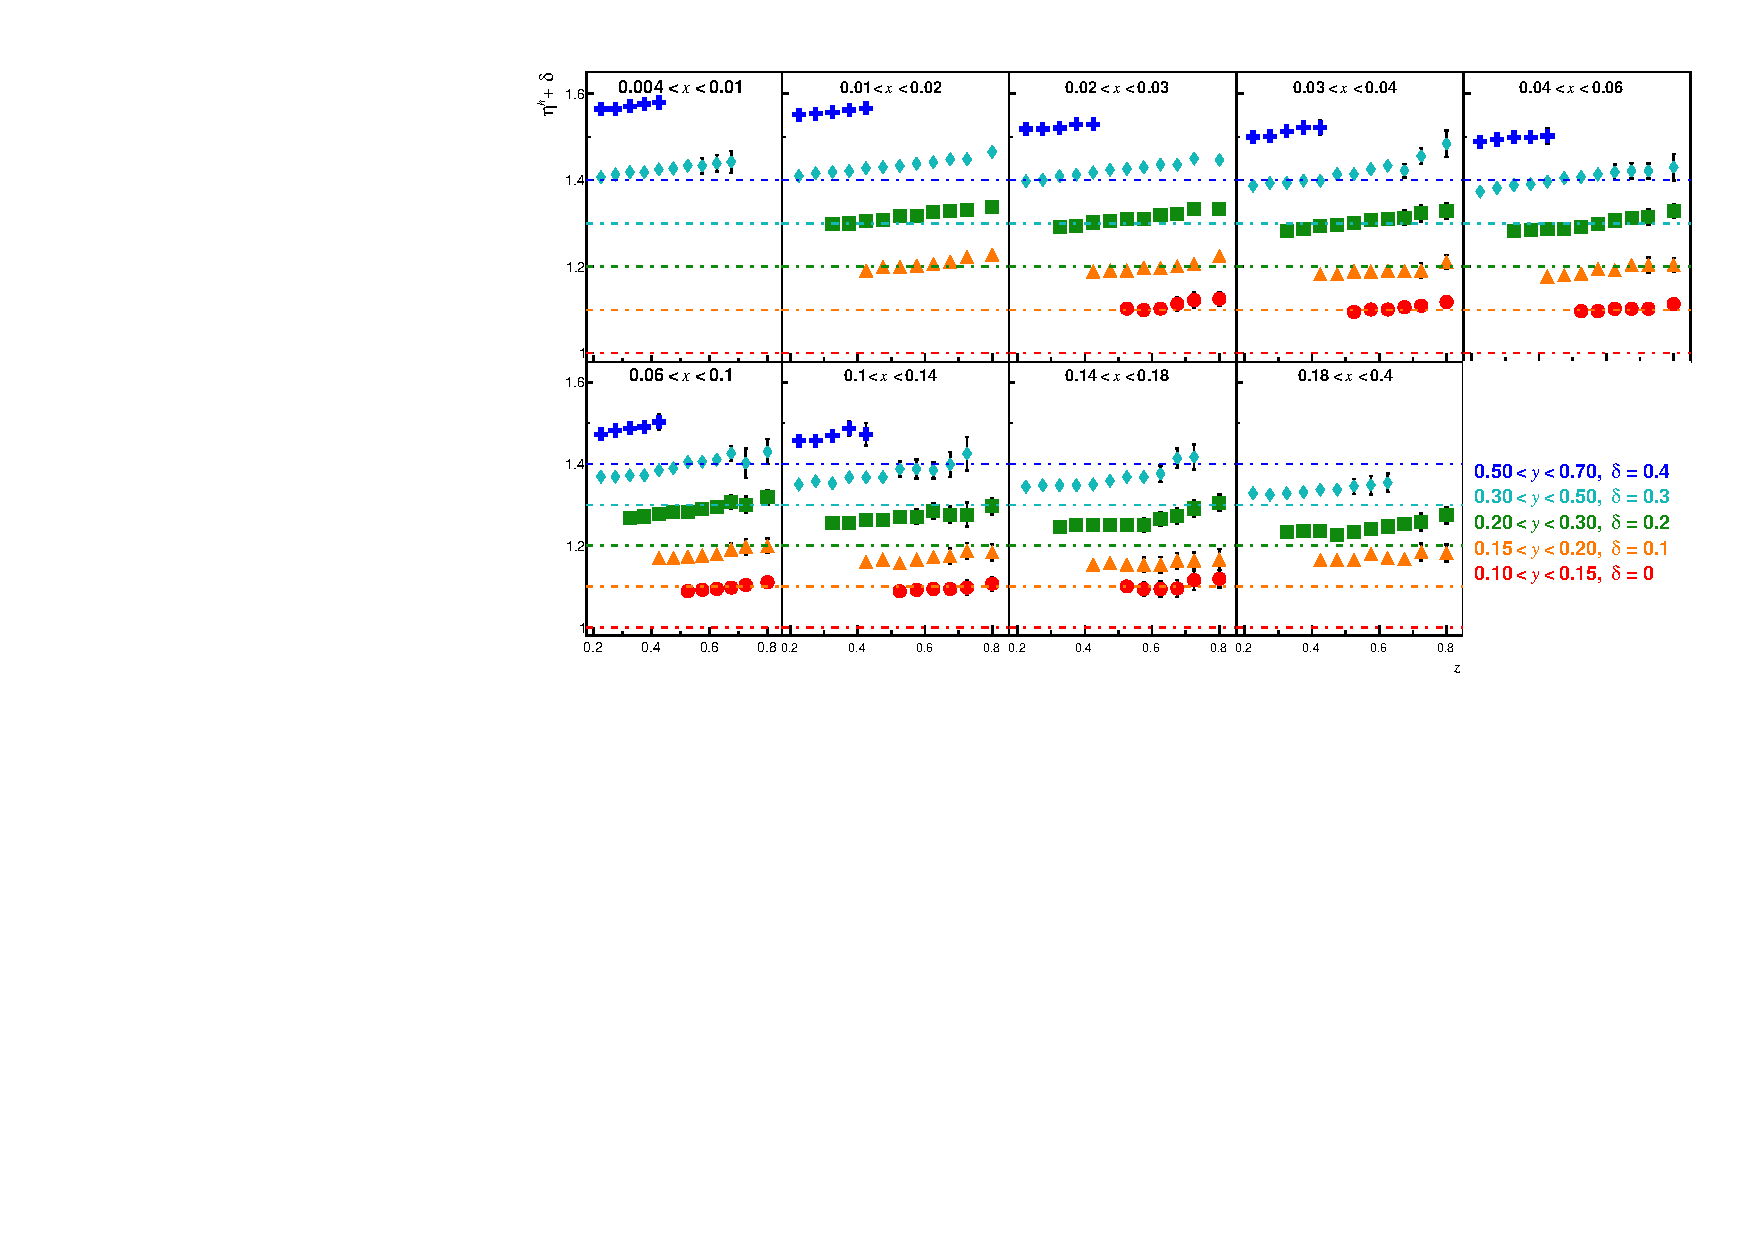
\epsfig{file=gfx/hadron_ratio.pdf,width=16cm}}
\caption{$\eta^{h^{\pm}}(x,y,z)$, positive hadrons in full points, negative in open points, in bins of $x$, staggered with $y$ and versus $z$.
The corrections go from $0$\% at low $z$ and low $y$ to 10\% at high $z$ and high $y$}\label{fig:hadz_ratio}
\end{figure}

%----------------------------------------------------------------------------------------

\section{Comparison between DJANGOH and TERAD}

In the next figures, DJANGOH results are compared with TERAD \cite{TERAD}. The two programs are using the same set of $F^{p}_{2}$ and $R$. This are the only inputs (apart from the process input ie. $\mu p$ scattering at 160 GeV muon energy) that need to be identical so that the comparison is relevant. One thing to be noted is that TERAD is using in addition $O(\alpha^2)$ corrections. They should have an impact on the cross-section of TERAD, but are negligible.

The first check for consistency done in Fig.~\ref{fig:BRy} is to compare the $\sigma_{Born}$ of both programs. Using the same input information on $F^{p}_{2}(x,Q2)$ and $R(x, Q^2)$ does not guarantee that $\sigma_{Born}$ for both program, called $\sigma^{D}_{Born}$ and $\sigma^{T}_{Born}$, is the same : the reason is that for example in TERAD, $\sigma^{T}_{Born}$ is computed without constants like $\pi$, $M_{proton}$, $\alpha$, etc. and its functional form is unknown, unlike in DJANGOH. This means that the ratio $r=\frac{\sigma^{D}_{Born}}{\sigma^{T}_{Born}}$ may differ from 1 but must be constant as a function of $x$ and $y$.

\begin{figure}[!htb]
\centerline{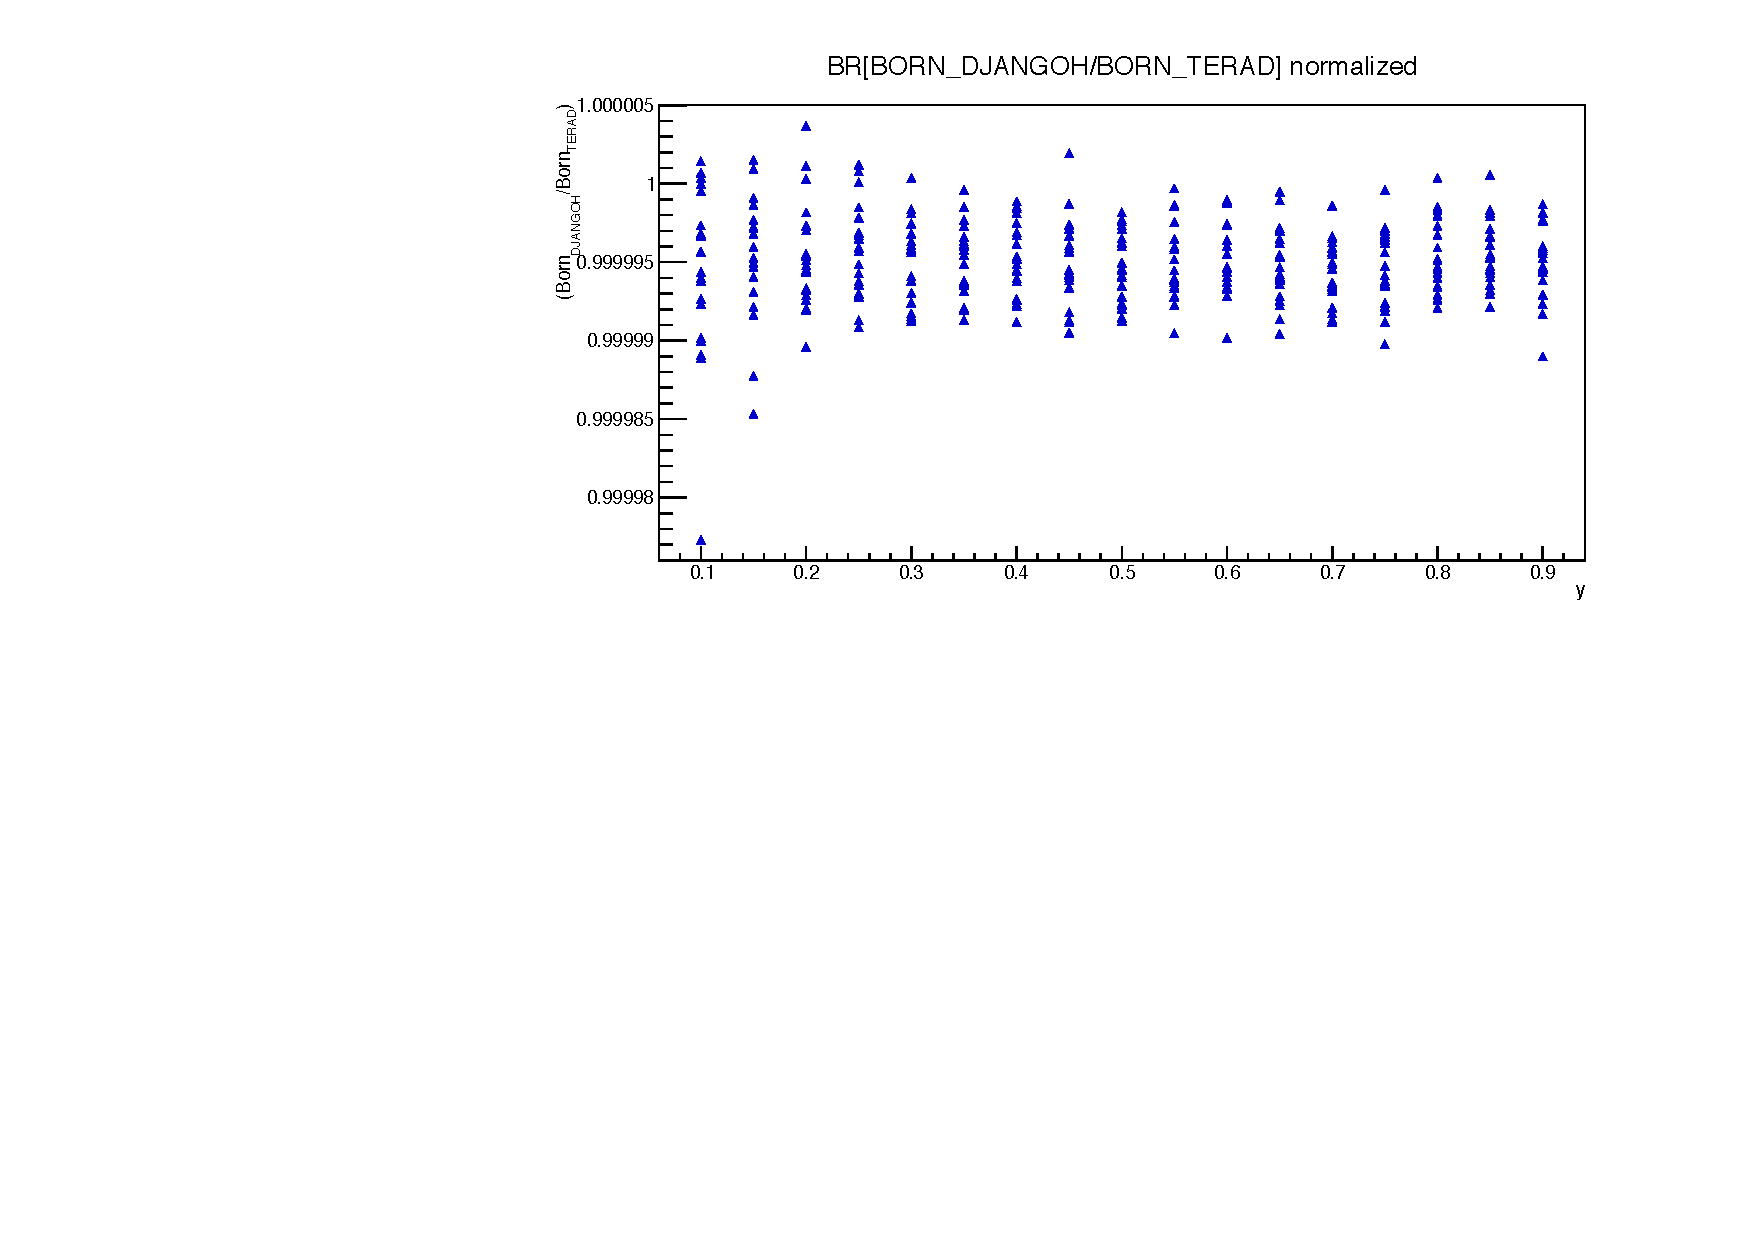
\epsfig{file=gfx/BRy.pdf,width=14cm}}
\caption{Ratio of the Born cross-sections calculated with DJANGOH and TERAD, for the same $F_2$ and $R$ parametrizations, as a function of $y$ at different values of $x$ (staggered points at fixed $y$)}\label{fig:BRy}
\end{figure}

The radiative correction factors $\eta(x,y)$ for DJANGOH ($\eta_D$) and TERAD ($\eta_T$) are compared in Fig.~\ref{fig:RCy}. The absolute difference is then plotted in Fig.~\ref{fig:ERy}, showing that the two programs differ at most $3$\% in the region of lowest $x$ and highest $y$. This results is extremely good, knowing that DJANGOH and TERAD are not using the same renormalization scheme.


\begin{figure}[htb]
\centerline{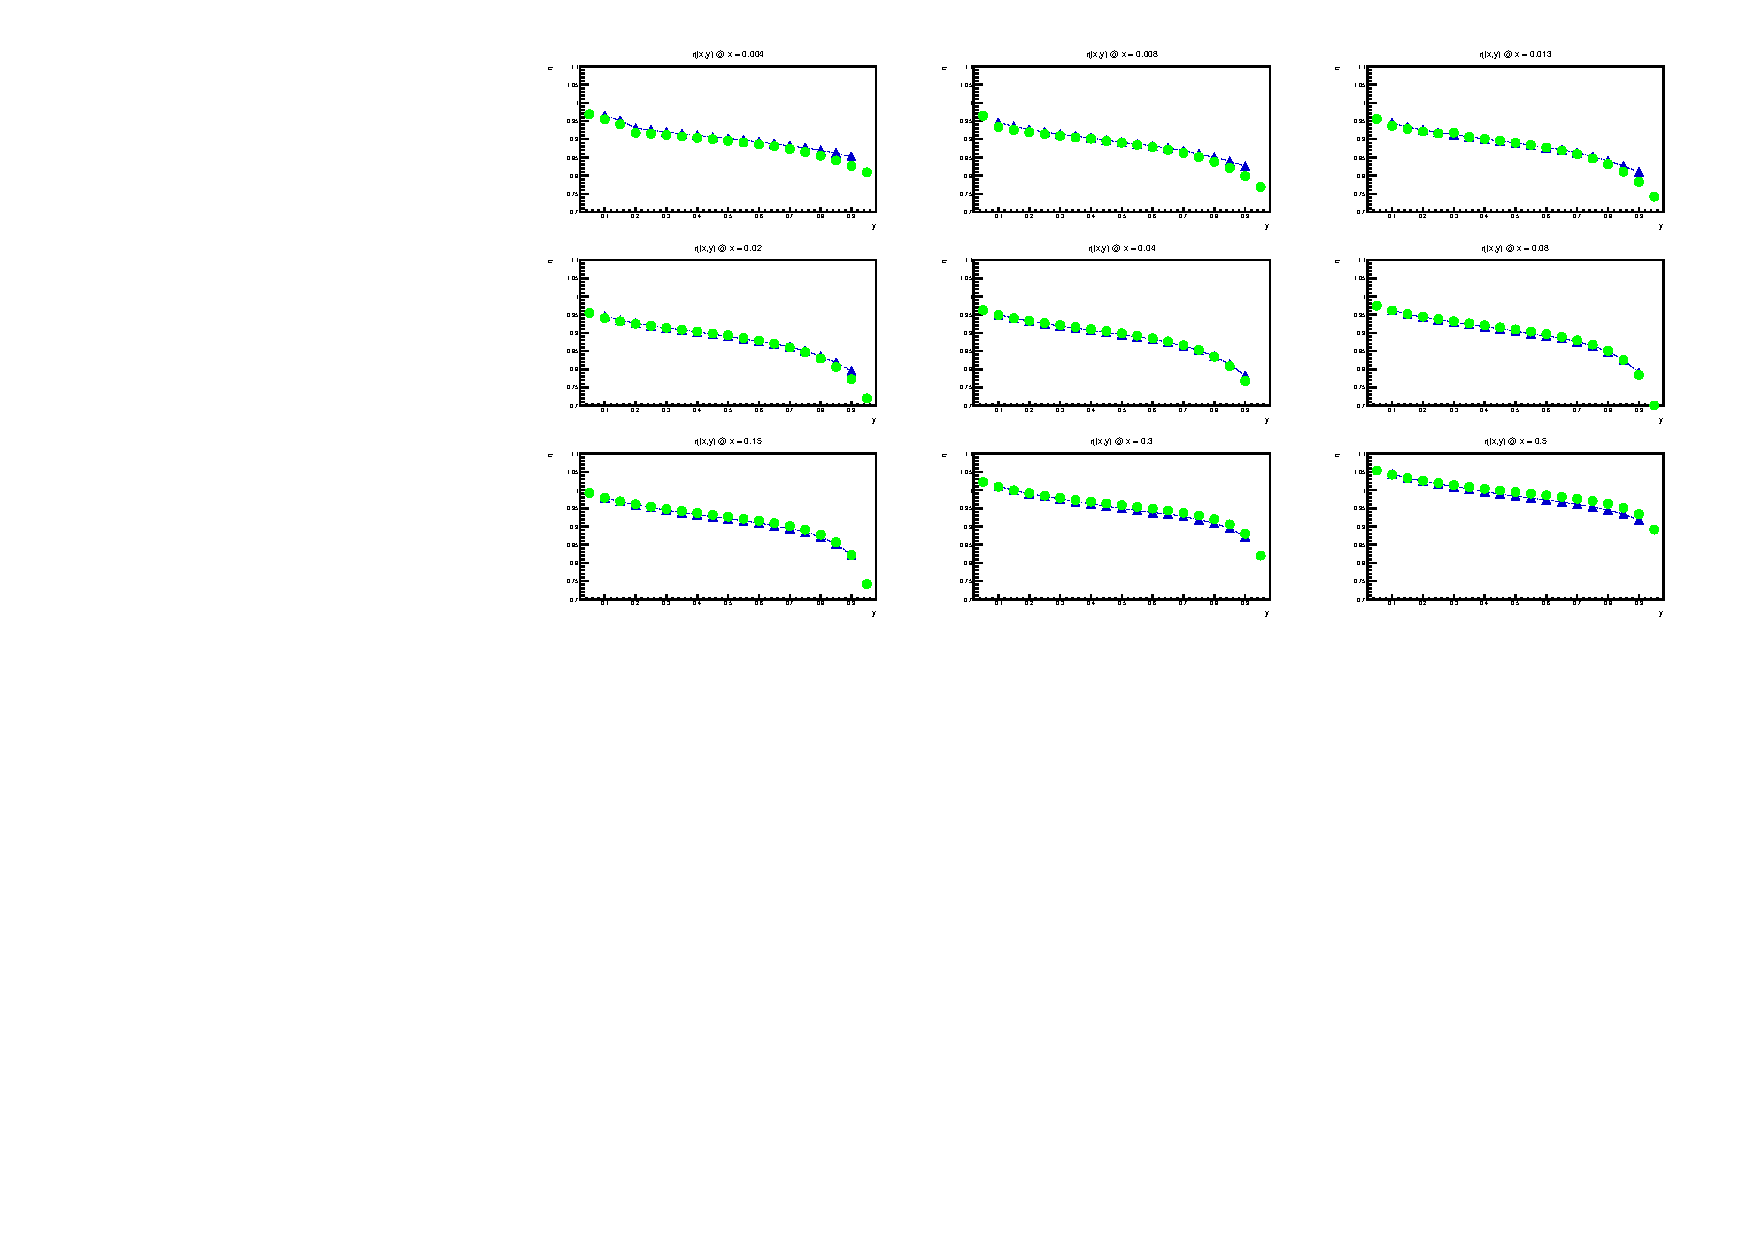
\epsfig{file=gfx/RCy.pdf,width=14cm}}
\caption{Comparison of radiative corrections factor $\eta(y)$ for fixed values of $x$, computed for proton target at 160 GeV and with the same $F^p_2$ and $R$ parametrizations. Green dots mark results of TERAD, blue triangles the results of DJANGOH.}\label{fig:RCy}
\end{figure}

\begin{figure}[htb]
\centerline{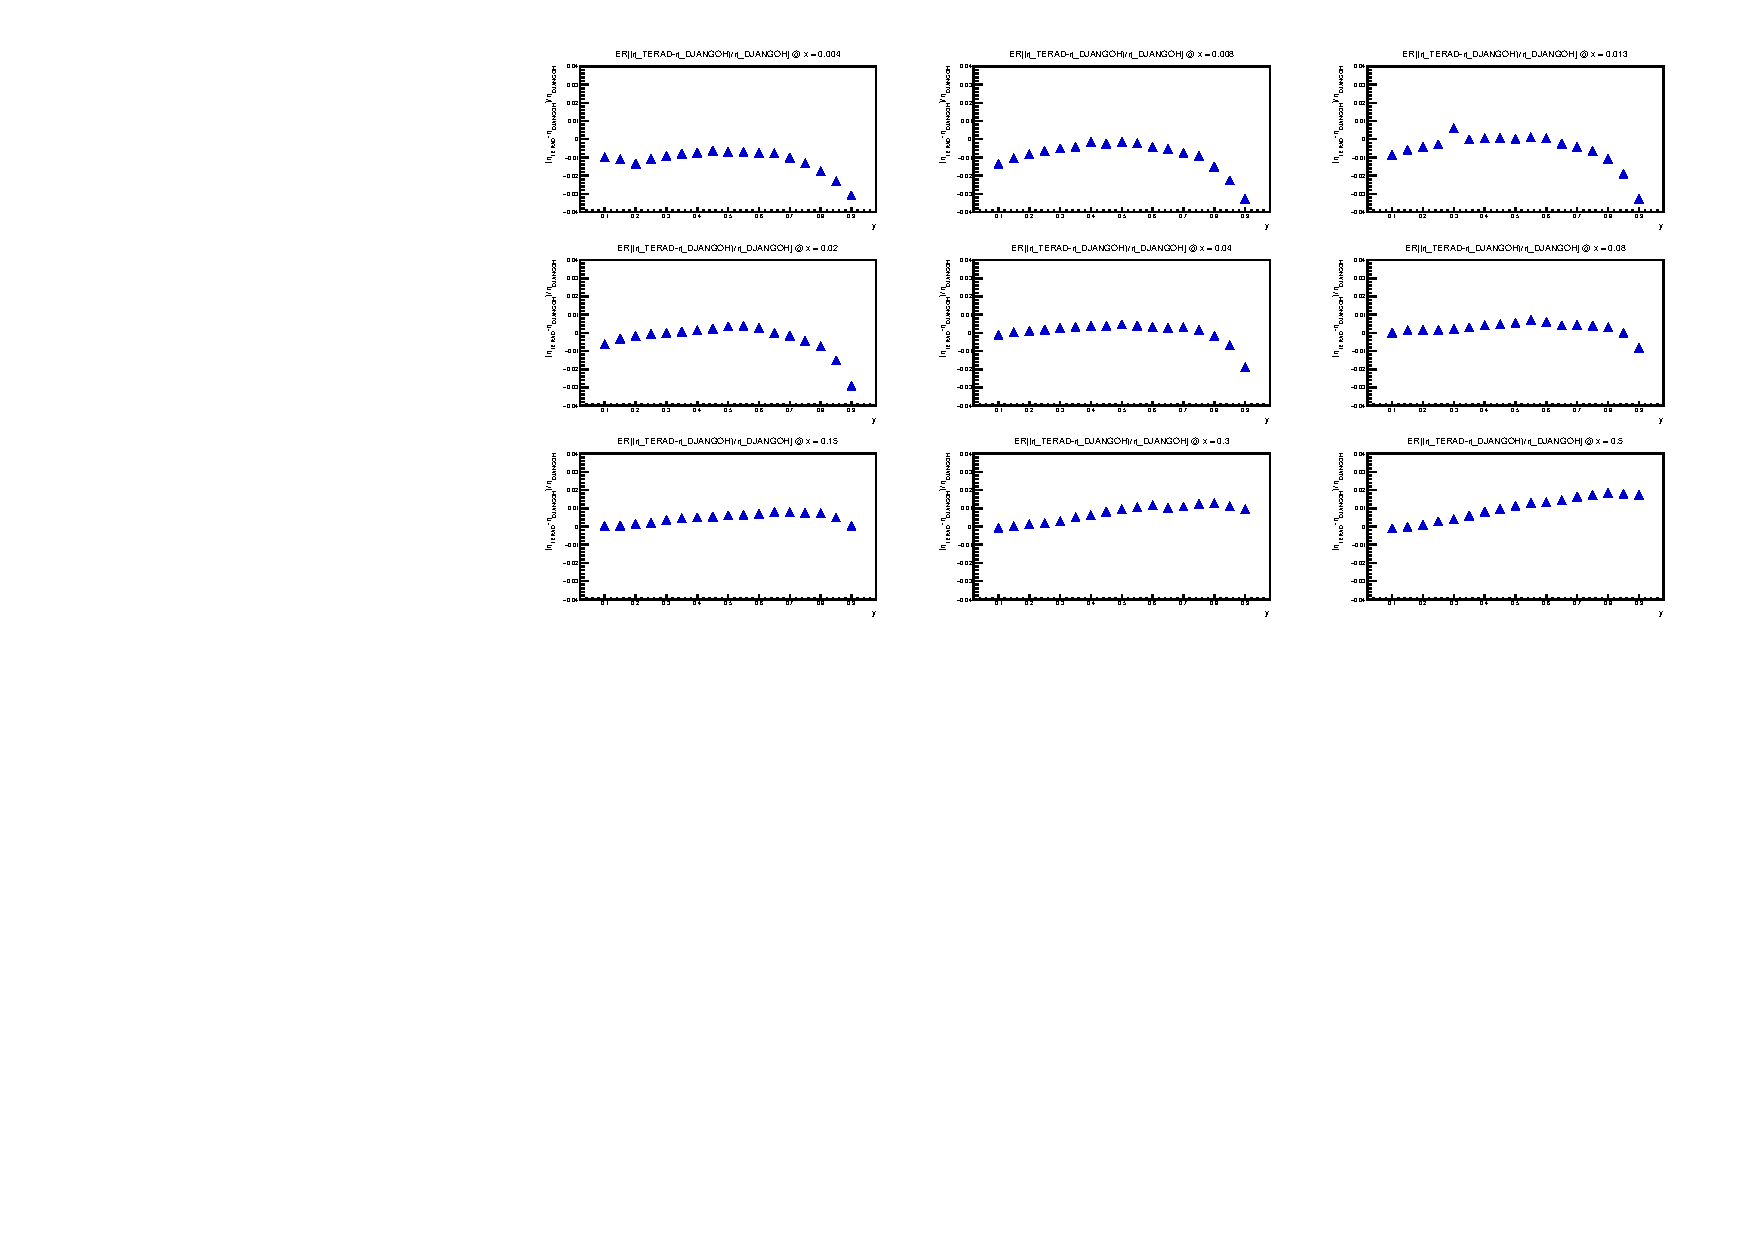
\epsfig{file=gfx/ERy_scat.pdf,width=14cm}}
\caption{Ratio of radiative corrections factors obtained in Fig~\ref{fig:RCy} $(\eta_T/\eta_D)-1$ as a function of $y$ for fixed values of $x$}\label{fig:ERy}
\end{figure}

\newpage

%----------------------------------------------------------------------------------------

\section{Summary}

The DJANGOH event generator with radiative events is a way to access radiative correction factor in a three dimensional ($x$,$y$,$z$) binning, like in the multiplicity analysis. This kind of correction are unprecedented for this analysis inside the COMPASS collaboration. The size of the correction, going from $0$ to $20$\% is within the expectations. Moreover, this correction can directly be applied on the multiplicities. When compared with TERAD computation on the inclusive corrections, the results of DJANGOH are shown to be compatible within $3$\%, a really good result knowing that DJANGOH and TERAD are not using the same renormalization scheme.
